\chapter{Оцінка і порівняння моделей}


У ході курсової роботи для оцінки та візуалізації моделей була створена 
програма, яка дозволяє користувачу регулювати параметри та одразу бачити, 
як вони впливають на прогнози. Також реалізована кнопка, яка починає 
оптимізацїю початкових параметрів, налаштованих користувачем, методом рою 
часток (одна з часток ініціалізована початковими параметрами). Також 
є опція зберегти параметри у форматі json. 
Основна програма написана на мові програмування Python, функції поделювання 
написані на C задля збільшення швидкості оптимізації.

\begin{figure}[H]
    \centering
    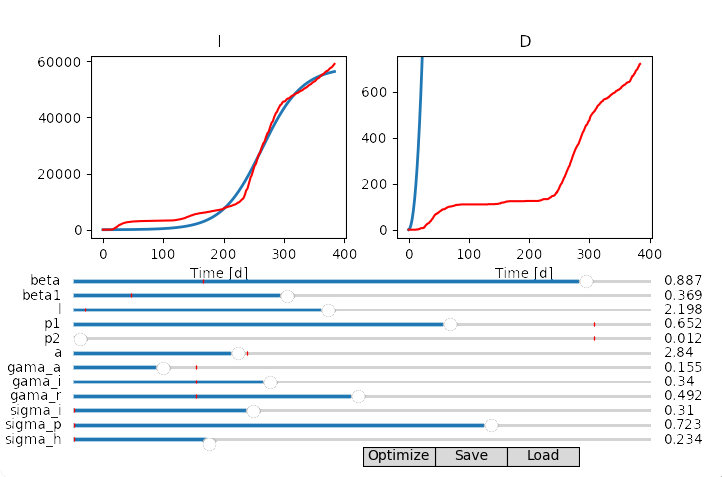
\includegraphics[scale=0.7]{program.png}
    \caption{Програма для підбору і оптимізації параметрів моделей}
    \label{fig:plot0}
\end{figure}


\section{Справжні дані та оцінка ефективності}

Прогнозувати будемо розвиток коронавірусу у Люксимбургу через те, що країна 
досить не велика та має середню густоту населення. 
Підбирати параметри будемо за перший рік епідемії і відповідний прогноз 
будемо робити на наступні двадцять днів. Для оцінки моделей будемо 
використовувати дві похибки, похибка моделювання - сума квадратів відстаней 
між графіками кожного дня (при кожному цілому $t$) і похибку прогнозування -
та сама величина але саме за давдцять днів прогнозування. 

\section{SIR}


SIR модель погано моделює навіть ту частину графіка, яку ми використали для 
налаштування її параметрів. Середня різниця між графіками на відрізку 
прогнозування (20 днів) має порядк сотень людей. 
Похибка моделювання - 36695055916, похибка прогнозування - 142262882.


\begin{figure}[H]
    \centering
    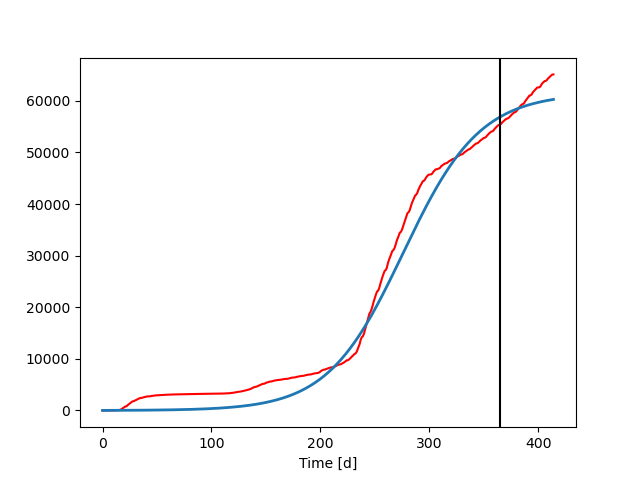
\includegraphics[scale=0.5]{SIR365.png}
    \caption{Прогноз SIR моделі після 365 днів}
    \label{fig:plot1}
\end{figure}


\section{SEIR}


З SEIR моделлю вже можливо досить непогано апроксимувати графік, проте 
прогноз і реальні дані мають зовсім різну динаміку, порядок похибки - 
тисячі, отже дану модель не можна використовувати для пронозів. 
Похибка моделювання 36697160718, похибка прогнозування 131123602.


\begin{figure}[H]
    \centering
    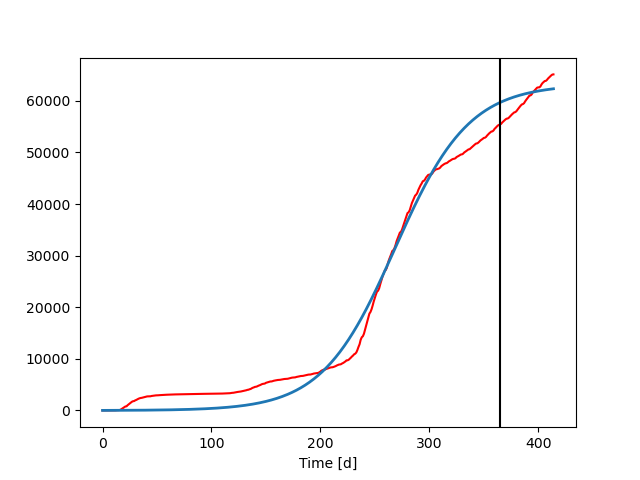
\includegraphics[scale=0.5]{SEIR365.png}
    \caption{Прогноз SEIR моделі після 365 днів}
    \label{fig:plot2}
\end{figure}
\section{SEIPR}

Модель має велику похибку на 365 день моделювання, через це прогноз 
на наступні дні має велику різницю з реальними данними. 
Похибка моделювання 36603451786, похибка прогнозування 241067088.

\begin{figure}[H]
    \centering
    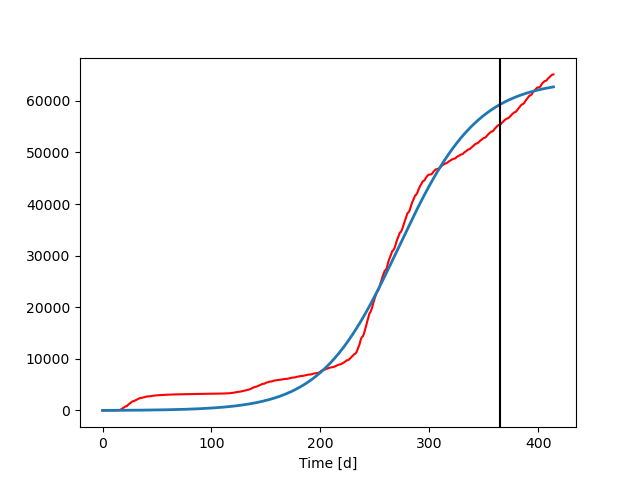
\includegraphics[scale=0.5]{SEIPR365.png}
    \caption{Прогноз SIPR моделі після 365 днів}
    \label{fig:plot3}
\end{figure}
\section{SEIAPR}

Модель краще апроксимує графік, проте все ще погано моделює 
кількість хворих на короткі періоди часу. 
Загальна похибка 36663218005
Похибка моделювання 36772792167, похибка прогнозування 107349315.
\begin{figure}[H]
    \centering
    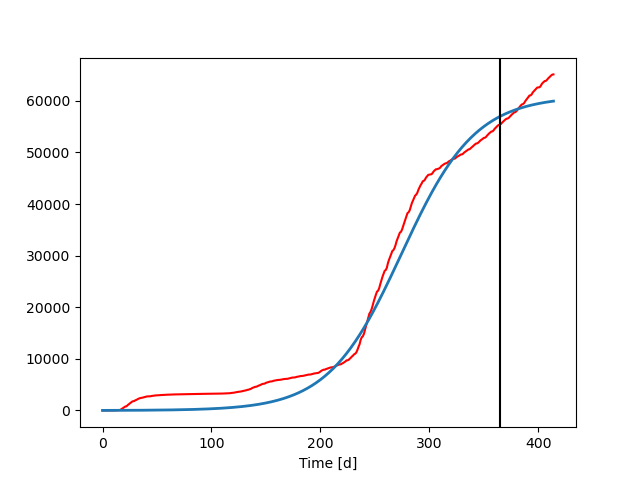
\includegraphics[scale=0.5]{SEIAPR365.png}
    \caption{Прогноз SEIAPR моделі після 365 днів}
    \label{fig:plot4}
\end{figure}
\section{SEIAPHRD}


Данна модель непогано апроксимує графік, проте початок у них досить сильно 
розбігається. Також сильно розбігаються графіки смертей та госпіталізованих.
Модель спромоглася зробити досить точний прогноз на декілька 
днів.
Похибка моделювання 2121319813, похибка прогнозування 40889031.
\begin{figure}[H]
    \centering
    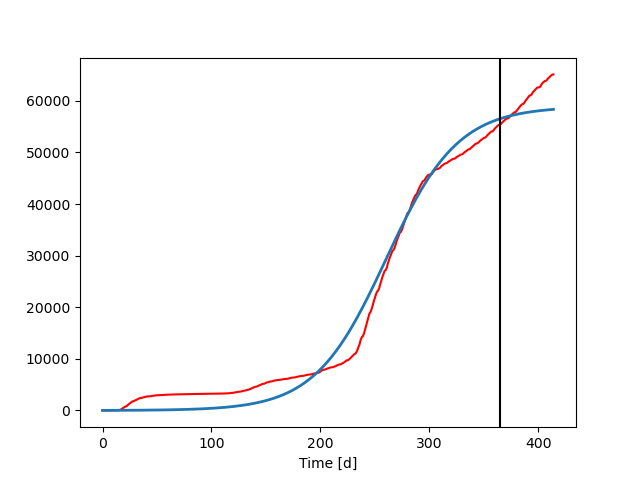
\includegraphics[scale=0.5]{model1_365.png}
    \caption{Прогноз SEIAPHRD моделі після 365 днів}
    \label{fig:plot5}
\end{figure}


\section{Порівняння моделей та результати}


В усіх моделей є проблеми з моделюванням початку епідемії та в місцях 
різкої зміни динаміки розвитку захворюваності. Можливо варто 
використовувати змінні параметри моделі або застосувати більш складну 
механіку захворювання. 
Не зважаючи на це моделі спроможні дати досить точний 
короткостроковий прогноз. 
Даля наведена таблиця для порівняння результатів. 

\begin{center}
    \begin{tabular}{||c c c c||} 
        \hline
        назва моделі & моделювання & 
        прогнозування & прогнозування 3 дні \\ [0.1ex] 
        \hline\hline
        SIR & 36695055916 & 142262882 & 787 \\ 
        \hline
        SEIR &  36697160718 & 131123602 & 5415 \\
        \hline
        SEIPR &  36603451786 & 241067088 & 7507 \\
        \hline
        SEIAPR &  36772792167 & 107349315 & 7560 \\
        \hline
        SEIAPHRD & 2121319813 & 40889031 & 6344 \\ [1ex] 
        \hline
    \end{tabular}
\end{center}